\documentclass[10pt,a4paper,twocolumn]{article}
% Shared preamble for the synthetic Turkish corpus (compiled with tectonic).
\usepackage{iftex}
\ifXeTeX
  \usepackage{fontspec} % Latin Modern OpenType, proper ToUnicode for Turkish letters
\else
  \usepackage[T1]{fontenc}
  \usepackage[utf8]{inputenc}
  \usepackage{lmodern}
\fi
\usepackage[turkish,shorthands=off]{babel}
\usepackage{amsmath,amssymb}
\usepackage{graphicx}
\usepackage{xcolor}
\usepackage{tikz}
\usepackage{booktabs}
\usepackage{hyperref}
\hypersetup{colorlinks=true,linkcolor=blue!50!black,urlcolor=blue!50!black,citecolor=green!40!black}
\newcommand{\paragrafA}{Makine çevirisi sistemleri son on yılda büyük bir gelişme göstermiştir. Özellikle sinir ağı tabanlı yöntemler, kelime düzeyinde değil tümce düzeyinde bağlamı dikkate alarak daha akıcı çeviriler üretmektedir. Bununla birlikte akademik metinlerde terimlerin tutarlı biçimde çevrilmesi, kesinlik derecesinin korunması ve sayısal değerlerin değiştirilmemesi hâlâ önemli sorunlar arasında yer almaktadır.}
\newcommand{\paragrafB}{Bu çalışmada 2019–2023 yılları arasında yayımlanmış 412 makaleden oluşan bir derlem kullanılmıştır. Her makale için özet, giriş ve sonuç bölümleri ayrı ayrı değerlendirilmiş; toplam 18.640 tümce iki bağımsız uzman tarafından incelenmiştir. Uzmanlar arasındaki uyum katsayısı $\kappa = 0{,}81$ olarak hesaplanmıştır.}
\newcommand{\paragrafC}{Bulgular, uzun ve iç içe geçmiş tümcelerde terim tutarlılığının belirgin biçimde azaldığını göstermektedir. Ortalama terim tutarlılığı \%87,4 olarak ölçülmüş; ancak kırk sözcükten uzun tümcelerde bu oran \%71,2'ye düşmüştür. Bu fark istatistiksel olarak anlamlıdır ($p < 0{,}01$).}

\usepackage[margin=1.8cm,columnsep=0.6cm]{geometry}
% Structures that broke the analysis of a real two-column paper (ADR-018 follow-up): a rotated
% margin stamp, a two-line centred title, superscript-led affiliation lines, a full-width table
% above column tables, consecutive booktabs tables (the second without a bottom rule) and a
% chart whose tick labels sit right above the axis title.
\begin{document}
\twocolumn[{\centering
{\LARGE\bfseries Akademik Metinlerin Makine Çevirisinde Anlam Kaymasını Ölçen Yeni Bir Yaklaşım\par}
\vspace{0.6em}
{\large Zeynep Kaya\textsuperscript{1}, Ahmet Demir\textsuperscript{2}\par}
\vspace{0.3em}
{\small\textsuperscript{1}Orta Doğu Teknik Üniversitesi, Ankara, Türkiye; zeynep@example.org\par
\textsuperscript{2}Boğaziçi Üniversitesi, İstanbul, Türkiye; ahmet@example.org\par}
\vspace{1.2em}}]
\begin{tikzpicture}[remember picture,overlay]
\node[rotate=90,anchor=north,text=gray] at ([xshift=0.9cm]current page.west) {\LARGE arXiv:2401.01234v1 [cs.CL] 2 Oca 2024};
\end{tikzpicture}
\section{Giriş}
\paragrafA\ \paragrafB\ \paragrafC\ \paragrafA
\section{Yöntem}
\paragrafB\ \paragrafC\ \paragrafA\ \paragrafB\ \paragrafC\ \paragrafA\ \paragrafB\ \paragrafC
\begin{table*}[t]
\centering
\caption{Tüm yapılandırmaların başarımı.}
\begin{tabular}{lrrrrrr}
\toprule
& \multicolumn{3}{c}{Genel} & \multicolumn{3}{c}{Sınıf başına} \\
\cmidrule(lr){2-4}\cmidrule(lr){5-7}
Girdi & Kesinlik & Duyarlılık & F1 & Kesinlik & Duyarlılık & F1 \\
\midrule
Metin & 97 & 83 & 89 & 96 & 67 & 79 \\
Metin + üstveri & 98 & 91 & 94 & 97 & 81 & 89 \\
\bottomrule
\end{tabular}
\end{table*}
\begin{table}[h]
\centering
\caption{Sınıflandırıcıların başarımı.}
\begin{tabular}{lrr}
\toprule
Sınıflandırıcı & P (\%) & R (\%) \\
\midrule
Rastgele orman & 97 & 83 \\
Karar ağacı & 89 & 89 \\
\bottomrule
\end{tabular}
\vspace{0.4em}
\caption{Eğitim ve test kümelerindeki başarım.}
\begin{tabular}{llr}
\toprule
Küme & Tür & Toplam \\
\midrule
Eğitim & popüler & 5.193 \\
\midrule
Test & tipik & 397 \\
 & zararlı & 143 \\
\end{tabular}
\vspace{1.4em}
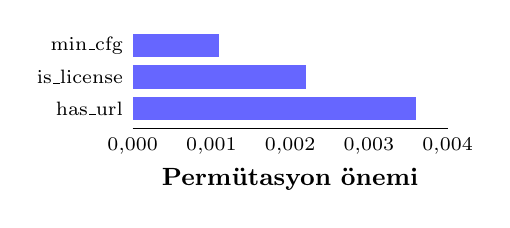
\begin{tikzpicture}
\foreach \y/\w/\name in {0/3.6/has\_url, 0.4/2.2/is\_license, 0.8/1.1/min\_cfg} {
  \fill[blue!60] (0,\y) rectangle (\w,\y+0.3);
  \node[left,font=\scriptsize] at (0,\y+0.15) {\name};
}
\draw (0,-0.1) -- (4,-0.1);
\foreach \x/\t in {0/{0,000}, 1/{0,001}, 2/{0,002}, 3/{0,003}, 4/{0,004}} {
  \node[below,font=\scriptsize] at (\x,-0.1) {\t};
}
\node[font=\small\bfseries] at (2,-0.75) {Permütasyon önemi};
\end{tikzpicture}
\caption{Özelliklerin permütasyon önemi.}
\end{table}
\section{Sonuç}
\paragrafC\ \paragrafA\ \paragrafB\ \paragrafC\ \paragrafA\ \paragrafB\ \paragrafC\ \paragrafA
\end{document}
